\chapter*{Preface}

\section*{A free and open-source calculus \ \scalebox{0.5}{\includegraphics{figures/CClicense.eps}}} 

First and foremost, this text is mostly an adaptation of two very excellent open-source textbooks:  {\em Active Calculus} by Dr. Matt Boelkins and {\em \apex Calculus} by Drs. Gregory Hartman, Brian Heinold, Troy Siemers, Dimplekumar Chalishajar, and Jennifer Bowen.  Both texts can be found at
\begin{center} \href{http://aimath.org/textbooks/approved-textbooks/}
{\texttt{http://aimath.org/textbooks/approved-textbooks/}}. \end{center} 
Dr. Boelkins also has a great blog for open source calculus at
\begin{center} \href{https://opencalculus.wordpress.com/}
{\texttt{https://opencalculus.wordpress.com/}}. \end{center} 
The authors of this text have combined sections, examples, and exercises from the above two texts along with some of their own content to generate this text.  The impetus for the creation of this text was to adopt an open-source textbook for Calculus while maintaining the typical schedule and content of the calculus sequence at our home institution.

Several fundamental ideas in calculus are more than 2000 years old.  As a formal subdiscipline of mathematics, calculus was first introduced and developed in the late 1600s, with key independent contributions from Sir Isaac Newton and Gottfried Wilhelm Leibniz.  Mathematicians agree that the subject has been understood rigorously since the work of Augustin Louis Cauchy and Karl Weierstrass in the mid 1800s when the field of modern analysis was developed, in part to make sense of the infinitely small quantities on which calculus rests.  Hence, as a body of knowledge calculus has been completely understood by experts for at least 150 years.  The discipline is one of our great human intellectual achievements:  among many spectacular ideas, calculus models how objects fall under the forces of gravity and wind resistance, explains how to compute areas and volumes of interesting shapes, enables us to work rigorously with infinitely small and infinitely large quantities, and connects the varying rates at which quantities change to the total change in the quantities themselves.

While each author of a calculus textbook certainly offers her own creative perspective on the subject, it is hardly the case that many of the ideas she presents are new.  Indeed, the mathematics community broadly agrees on what the main ideas of calculus are, as well as their justification and their importance; the core parts of nearly all calculus textbooks are very similar.  As such, it is our opinion that in the 21st century -- an age where the internet permits seamless and immediate transmission of information -- no one should be required to purchase a calculus text to read, to use for a class, or to find a coherent collection of problems to solve.  Calculus belongs to humankind, not any individual author or publishing company.  Thus, the main purpose of this work is to present a new calculus text that is \emph{free}.  In addition, instructors who are looking for a calculus text should have the opportunity to download the source files and make modifications that they see fit; thus this text is \emph{open-source}.  

Because the text is free and open-source, any professor or student may use and/or change the electronic version of the text for no charge.  Presently, a .pdf copy of the text and its source files may be obtained by download from Github (insert link here!!)
%\begin{center} \href{http://faculty.gvsu.edu/boelkinm/Home/Download.html}{\texttt{http://faculty.gvsu.edu/boelkinm/Home/Download.html}}. 
%\end{center}  
This work is licensed under the Creative Commons Attribution-NonCommercial-ShareAlike 4.0 Unported License.  The graphic 
\begin{center}
\includegraphics{figures/CClicense.eps}
\end{center}
that appears throughout the text shows that the work is licensed with the Creative Commons, that the work may be used for free by any party so long as attribution is given to the author(s), that the work and its derivatives are used in the spirit of ``share and share alike,'' and that no party may sell this work or any of its derivatives for profit, with the following exception:  \emph{it is entirely acceptable for university bookstores to sell bound photocopied copies to students at their standard markup above the copying expense.}  Full details may be found by visiting
\begin{center}
\href{http://creativecommons.org/licenses/by-nc-sa/4.0/}{\texttt{http://creativecommons.org/licenses/by-nc-sa/4.0/}}
\end{center} 
or sending a letter to Creative Commons, 444 Castro Street, Suite 900, Mountain View, California, 94041, USA. 

\section*{Acknowledgments}

We would like to thank Affordable Learning Georgia for awarding us a Textbook Transformation Grant, which allotted a two-course release for each of us to generate this text.  Please see
\begin{center}
\href{http://affordablelearninggeorgia.org/}{\texttt{http://affordablelearninggeorgia.org/}}
\end{center} 
for more information on this initiative to promote student success by providing affordable textbook alternatives.

We will gladly take reader and user feedback to correct them, along with other suggestions to improve the text. \\

\ \hfill Jared Schlieper \& Michael Tiemeyer
 
